\paragraph{\trDonaldson--\trFukayaCategory。}\label{sub:donaldson-fukaya-category}
一个普遍的事实是：人们可以对任何\trOpenString{} TQFT 联系上一个\trFrobenius\trCategory。在%
\trFloer{}理论的语境中，这给出一个 $\KK$-\trLinear\trCategory{}$H\scr{F}(M)^{\mathrm{pr}}$，
称为（初步版本的）\trDonaldson--\trFukayaCategory。\trObject{}是\trExact\trLagrange\trSubmanifold%
$L\subset M$。从 $L_0$ 到 $L_1$ 的\trMorphism{}空间是\trFloer{}群 $HF^{\mathrm{pr}}(L_0,L_1)$。
\trComposition
\begin{equation}\label{eq:triangle-product}
HF^{\mathrm{pr}}(L_1,L_2)\otimes HF^{\mathrm{pr}}(L_0,L_1)
\longrightarrow HF^{\mathrm{pr}}(L_0,L_2)
\end{equation}
是\textbf{\trTriangleProduct}（triangle product），用 TQFT 的话说，它就是\trInvariant{}$\Phi_S$，
其中%
$S$ 是去掉三个边界点（一个\trIncomingPoint、两个\trOutgoingPoint）并标以 $L_0$、$L_1$、$L_2$
的\trDisk。恒等\trMorphism{}是 $\Phi_H\in HF^{\mathrm{pr}}(L,L)$，我们把\trLabel{}$L$ 放在
$\partial H$ 上。\trComposition{}的结合性，以及 $\Phi_H$ 是一个单位元这一事实，都由 TQFT 的%
\trGluing{}公理得到。
\begin{figure}[htbp]
\centering
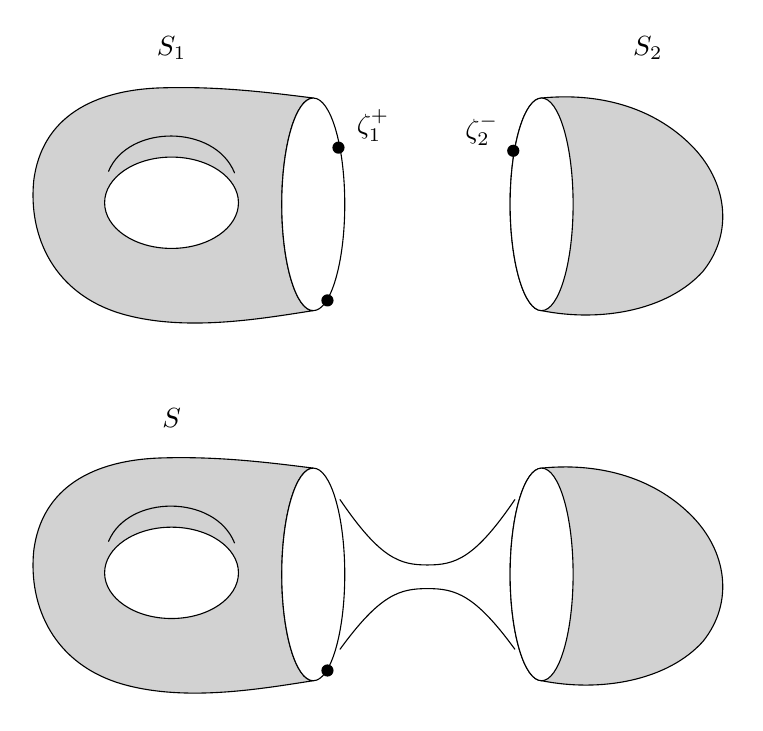
\begin{tikzpicture}[line cap=round,line join=round]
\draw[fill=gray!35]
  (3.10,1.35)
  .. controls (2.55,1.42) and (1.90,1.50) .. (1.20,1.48)
  .. controls (0.30,1.46) and (-0.35,1.10) .. (-0.45,0.30)
  .. controls (-0.52,-0.40) and (-0.20,-1.15) .. (0.70,-1.40)
  .. controls (1.50,-1.62) and (2.45,-1.45) .. (3.10,-1.35)
  arc (270:90:0.40 and 1.35) -- cycle;
\fill[white] (1.30,0.02) ellipse (0.85 and 0.58);
\draw (1.30,0.02) ellipse (0.85 and 0.58);
\draw (0.50,0.42) .. controls (0.75,1.02) and (1.85,1.02) .. (2.10,0.40);
\fill[white] (3.10,0) ellipse (0.40 and 1.35);
\draw (3.10,0) ellipse (0.40 and 1.35);
\fill (3.42,0.72) circle (2.2pt);
\fill (3.28,-1.22) circle (2.2pt);
\node at (3.86,1.00) {$\zeta_1^+$};
\draw[fill=gray!35]
  (6.00,-1.35)
  .. controls (6.75,-1.50) and (7.60,-1.35) .. (8.05,-0.85)
  .. controls (8.45,-0.35) and (8.35,0.30) .. (7.90,0.75)
  .. controls (7.40,1.25) and (6.70,1.42) .. (6.00,1.35)
  arc (90:270:0.40 and 1.35) -- cycle;
\fill[white] (6.00,0) ellipse (0.40 and 1.35);
\draw (6.00,0) ellipse (0.40 and 1.35);
\fill (5.64,0.68) circle (2.2pt);
\node at (5.24,0.94) {$\zeta_2^-$};
\node at (1.30,1.98) {$S_1$};
\node at (7.35,1.98) {$S_2$};
\begin{scope}[yshift=-4.7cm]
\draw (3.44,0.95) .. controls (3.95,0.20) and (4.20,0.12) .. (4.55,0.12)
      .. controls (4.90,0.12) and (5.15,0.20) .. (5.66,0.95);
\draw (3.44,-0.95) .. controls (3.95,-0.25) and (4.20,-0.18) .. (4.55,-0.18)
      .. controls (4.90,-0.18) and (5.15,-0.25) .. (5.66,-0.95);
\draw[fill=gray!35]
  (3.10,1.35)
  .. controls (2.55,1.42) and (1.90,1.50) .. (1.20,1.48)
  .. controls (0.30,1.46) and (-0.35,1.10) .. (-0.45,0.30)
  .. controls (-0.52,-0.40) and (-0.20,-1.15) .. (0.70,-1.40)
  .. controls (1.50,-1.62) and (2.45,-1.45) .. (3.10,-1.35)
  arc (270:90:0.40 and 1.35) -- cycle;
\fill[white] (1.30,0.02) ellipse (0.85 and 0.58);
\draw (1.30,0.02) ellipse (0.85 and 0.58);
\draw (0.50,0.42) .. controls (0.75,1.02) and (1.85,1.02) .. (2.10,0.40);
\draw[fill=gray!35]
  (6.00,-1.35)
  .. controls (6.75,-1.50) and (7.60,-1.35) .. (8.05,-0.85)
  .. controls (8.45,-0.35) and (8.35,0.30) .. (7.90,0.75)
  .. controls (7.40,1.25) and (6.70,1.42) .. (6.00,1.35)
  arc (90:270:0.40 and 1.35) -- cycle;
\fill[white] (3.10,0) ellipse (0.40 and 1.35);
\draw (3.10,0) ellipse (0.40 and 1.35);
\fill[white] (6.00,0) ellipse (0.40 and 1.35);
\draw (6.00,0) ellipse (0.40 and 1.35);
\fill (3.28,-1.22) circle (2.2pt);
\node at (1.30,1.98) {$S$};
\end{scope}
\end{tikzpicture}
\caption{}\label{fig:gluing-surfaces}
\end{figure}
$H\scr{F}(M)^{\mathrm{pr}}$ 的\trFrobenius{}性质如下。对每个 $L$，\trInvariant{}$\Phi_{\overline{H}}$
给出一个\trLinear{}映射 $HF^{\mathrm{pr}}(L,L)\to\KK$，把它与\trComposition{}相结合，就对任意
$L_0$、$L_1$ 得到一个\trNondegenerate\trPairing
$HF^{\mathrm{pr}}(L_1,L_0)\otimes_\KK HF^{\mathrm{pr}}(L_0,L_1)\to\KK$。更直接地说，定义这个%
\trPairing{}的\trSurface{}是一条带两个无穷远\trOutgoingPoint{}的无限\trStrip。通过粘贴这样的%
\trStrip，可以把无穷远\trIncomingPoint{}换成\trOutgoingPoint。这意味着两类点之间的区分在某种程度上
是人为的。人们固然可以把它取消（这样一来公理体系便与 TQFT 的原始表述 [7] 看齐），但由于一些在此后
会变得清楚的技术理由，我们不愿这样做。
我们还应当提到两条更特别属于\trDonaldson--\trFukayaCategory{}的性质。第一，对任何 $L$，都存在%
\trFrobenius{}代数的一个\trCanonical\trIsomorphism，即\trPiunikhin--\trSalamon--\trSchwarz
（PSS）映射 [106]
\begin{equation}\label{eq:pss-map}
H^*(L;\KK)\cong HF^{\mathrm{pr}}(L,L).
\end{equation}
理解\eqref{eq:pss-map} 的最好方式，是把它看作 TQFT 框架的一个自然推广的一部分：在这个推广里，
\trSurface{}$S$ 带有附加的标记边界点，而这些点随后以类似于\trGromov--\trWitten{}理论的方式处理。
其次，\trExact\trLagrange\trSubmanifold{}的每个\trIsotopy{}$\{L_s\}_{0\le s\le 1}$ 都在
$HF^{\mathrm{pr}}(L_0,L_1)$ 中给出一个特异元素，它具有如下性质：它只依赖于 $\{L_s\}$ 相对端点的%
\trHomotopy{}类；对常值\trIsotopy{}它就是恒等元素；而且\trIsotopy{}的\trComposition{}（作为路径）
对应于把
相应的元素取\trTriangleProduct。作为直接推论，所有这些元素都是 $H\scr{F}(M)^{\mathrm{pr}}$ 中的%
\trIsomorphism。由此可知，相互\trIsotopy{}的\trLagrange\trSubmanifold{}给出%
\trDonaldson--\trFukayaCategory{}中相互\trIsomorphic{}的\trObject，从而\trFloerCohomology{}群在%
\trIsotopy{}下不变。形式上，这一构造基于基本 TQFT 结构的又一种扩张，在其中容许%
\trLagrange\trBoundaryCondition{}沿 $\partial S$ 的诸点\trSmooth{}地变动。
